\section{Руководство пользователя}

\subsection{Назначение программы}

Разработанная программа реализует алгоритм сжатия изображений, повторяющий основные этапы стандарта JPEG. 
В отличие от оригинального алгоритма, на этапе энтропийного кодирования используется метод RLE (Run-Length Encoding) 
вместо кодирования по Хаффману. 
Это позволяет упростить реализацию, сохранив при этом все основные свойства алгоритма JPEG.

Программа предназначена для демонстрации полного цикла кодирования и декодирования изображения:

\begin{itemize}
    \item переход от $\textbf{RGB}$ к $\textbf{YCbCr}$
    \item разбиение на блоки $8 \times 8$
    \item дискретное косинус-преобразование (DCT)
    \item квантование
    \item последовательное сканирование (зигзаг)
    \item кодирование RLE
    \item обратные преобразования (IDCT и т. д.)
    \item восстановление RGB-изображения

\end{itemize}



\clearpage
%%%%%%%%%%%%%%%%%%%%%%%%%%%%%%%%%%%%%%%%%%%%%%%%
\subsection{Интерфейс программы}

На рисунке ~\ref{fig:interface} представлено главное окно приложения.

\begin{figure}[h!]
    \centering
    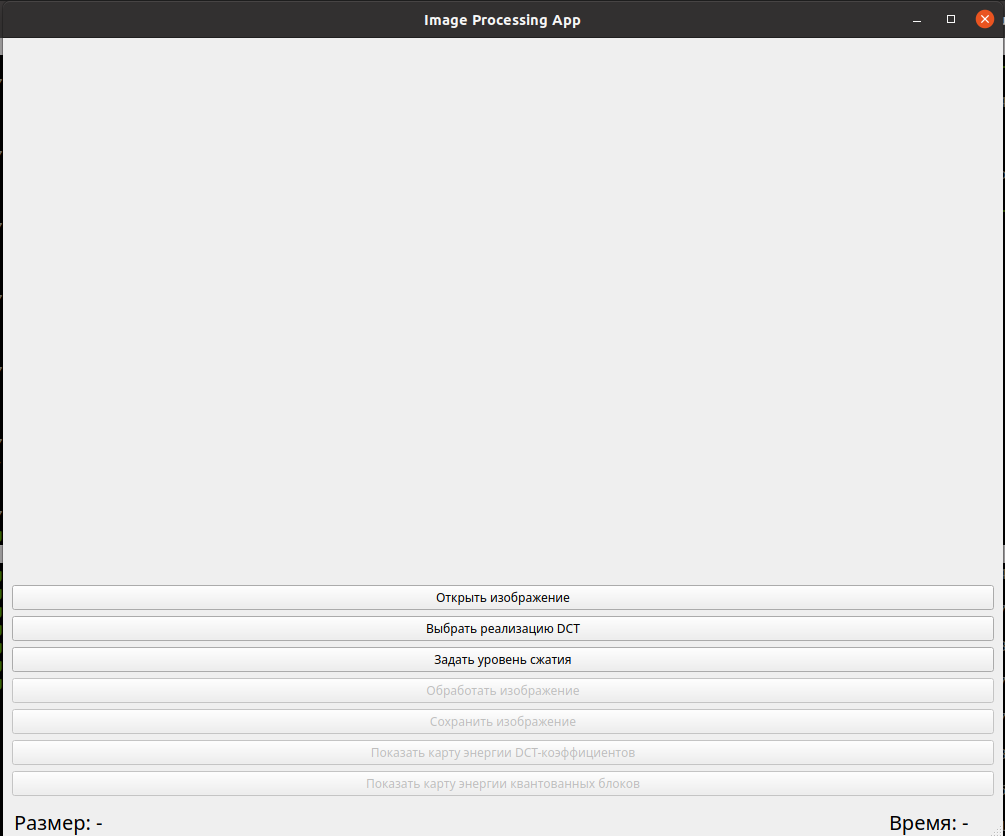
\includegraphics[width=0.7\textwidth]{/home/evgen/Coursework/app/diplom/images/interface.png}
    \caption{Главное окно приложения.}
    \label{fig:interface}
\end{figure}



\subsubsection{Основные элементы интерфейса:}

\begin{itemize}
    \item \textbf{Открыть изображение}

    Позволяет выбрать изображение в формате PNG или JPEG для обработки.
    
    \begin{figure}[h!]
        \centering
        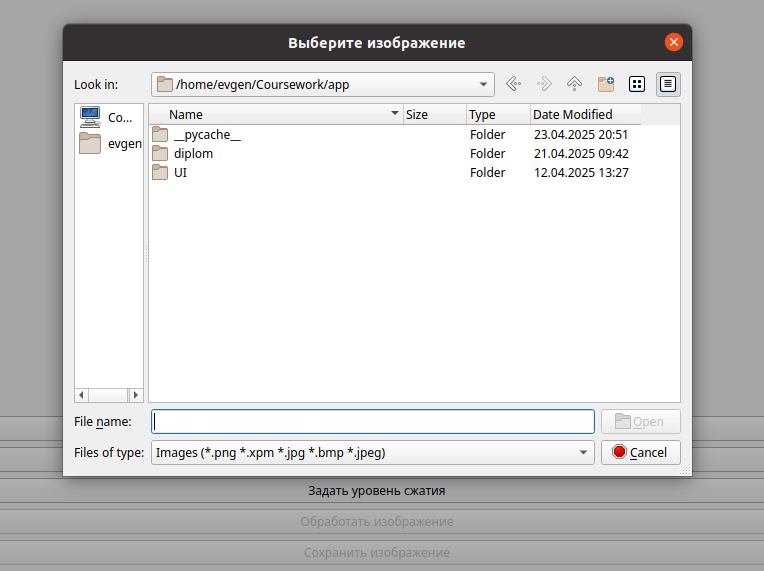
\includegraphics[width=0.5\textwidth]{/home/evgen/Coursework/app/diplom/images/win_choice.png}
        \caption{Окно выбора изображений.}
        \label{fig:win_choice}
    \end{figure}



    \item \textbf{Выбрать реализацию DCT}

    В графическом интерфейсе приложения предусмотрена возможность выбора реализации дискретного косинусного преобразования (DCT). 
    Пользователю предлагаются два варианта:

    Собственная реализация DCT, разработанная вручную в рамках дипломного проекта;
    
    Готовая реализация из библиотеки SciPy (scipy.fftpack.dct), используемая в качестве эталонной и производительной альтернативы.
    
    Это позволяет провести наглядное сравнение корректности и эффективности обеих реализаций, а также удостовериться в соответствии собственной реализации общепринятым стандартам.

    \begin{figure}[h!]
        \centering
        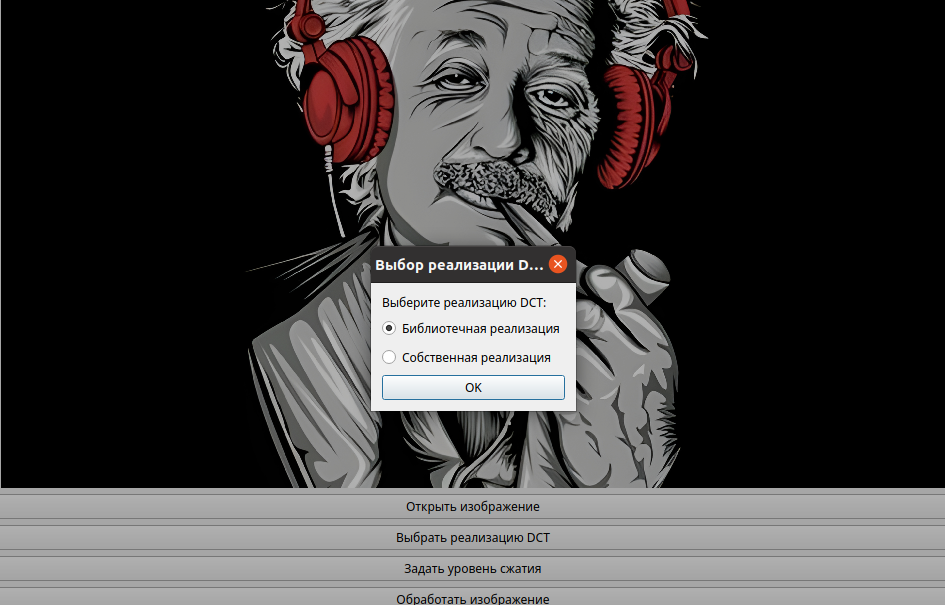
\includegraphics[width=0.8\textwidth]{/home/evgen/Coursework/app/diplom/images/choice_dct.png}
        \caption{Выбрать реализацию DCT.}
        \label{fig:choice_dct}
    \end{figure}





\end{itemize}



% Задать уровень сжатия — определяет степень квантования, влияя на степень потери информации и размер выходного файла.

% Обработать изображение — запускает основной процесс кодирования: преобразование, сжатие, RLE.

% Сохранить изображение — позволяет сохранить результат кодирования в файл.

% Показать карту энергии DCT-коэффициентов — визуализирует вклад разных частот в изображении до квантования.

% Показать карту энергии квантованных блоков — визуализирует энергию после квантования, демонстрируя потерю информации.

% В нижней части окна отображаются параметры:

% Размер — показывает размер обработанного изображения;

% Время — указывает, сколько времени занял процесс обработки.